\documentclass[../ManualeUtente.tex]{subfiles}
\begin{document}
	\section{Guida all'utilizzo}
		Di seguito è presentata una guida all'utilizzo di \progetto.\\
		I termini evidenziati in \textit{\textbf{questo modo}} corrispondono a pulsanti presenti all'interno
		dell'applicazione.
		\subsection{Interfaccia grafica}
			All'avvio dell'applicazione viene presentata una schermata come in Figura \ref{fig:StartScreen}.
			\begin{figure} [h!]
				\centering
				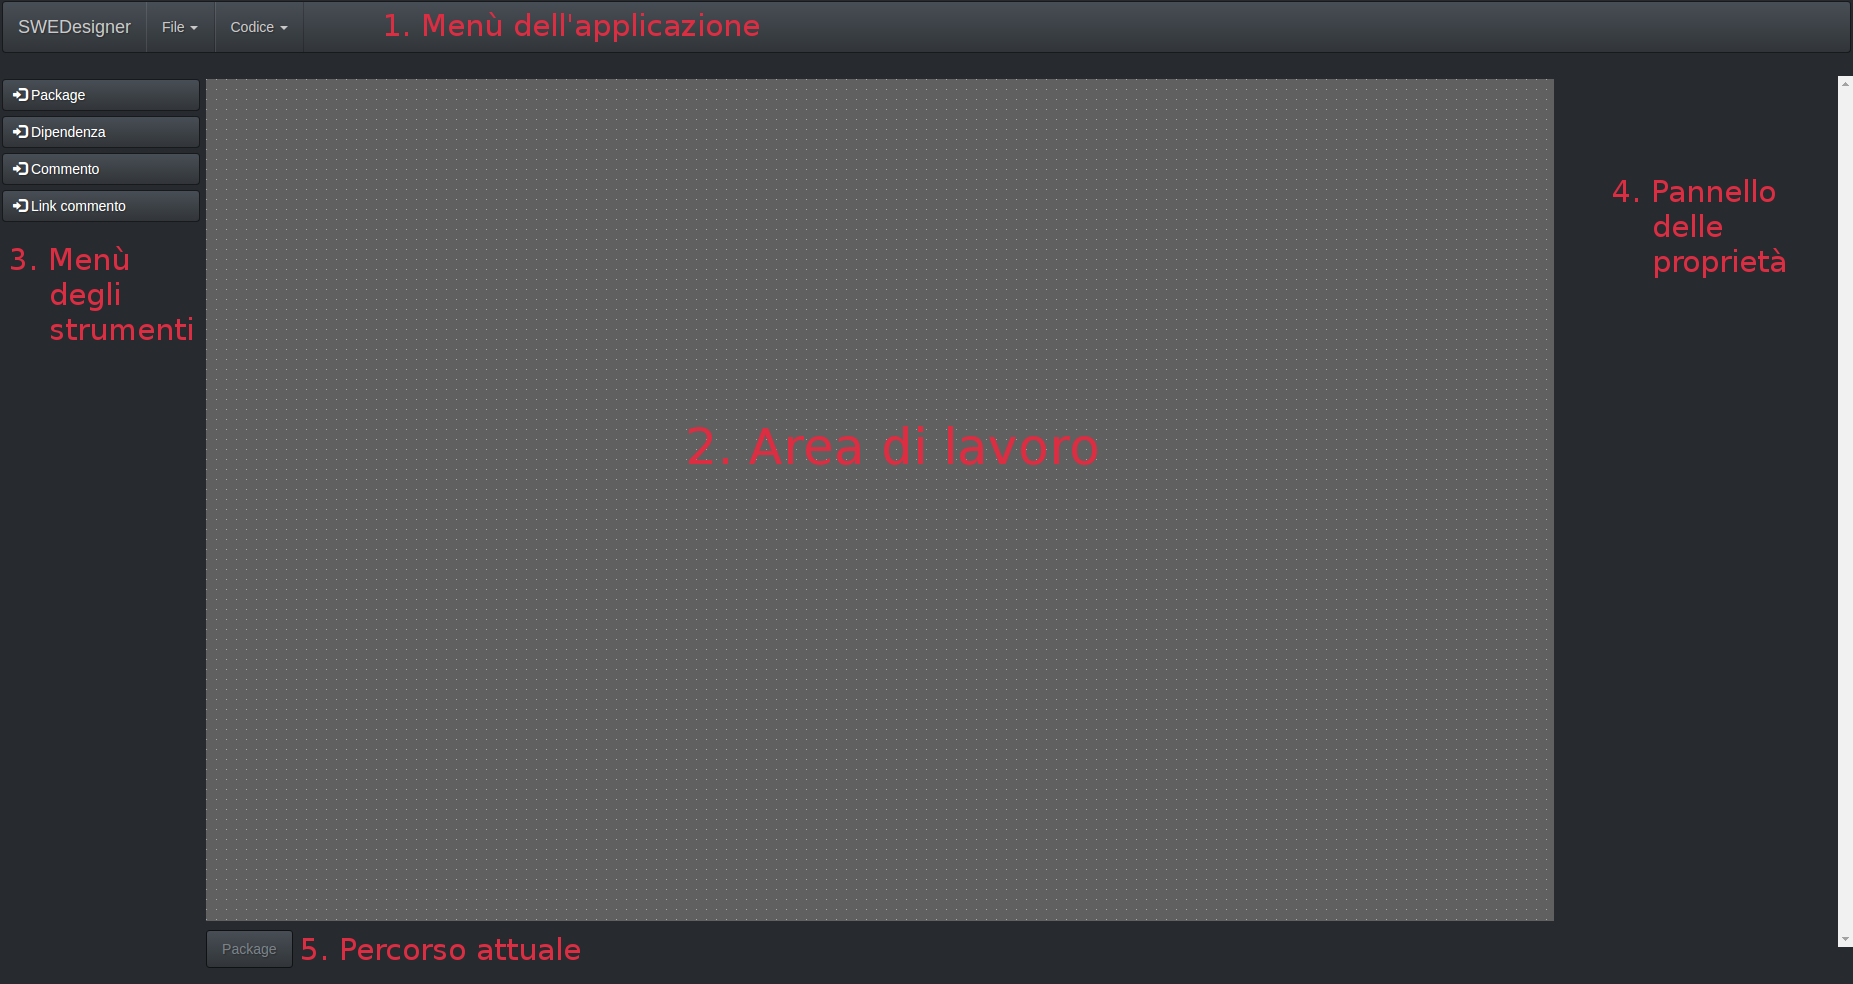
\includegraphics[scale=0.24]{./Immagini/StartScreen.png}
				\caption{Interfaccia grafica - Schermata iniziale}\label{fig:StartScreen}
			\end{figure}
			Ciò indica che è già stato aperto un nuovo progetto in cui è visualizzato il diagramma dei package vuoto ed è
			quindi possibile iniziare immediatamente a progettare il proprio programma.\\
			Dovunque vi troverete all'interno di \progetto, l'interfaccia grafica sarà
			sempre generalmente composta dalle seguenti componenti:
			\begin{enumerate}
				\item \underline{Menù dell'applicazione} situato nella parte superiore della schermata, dal quale è
				possibile interagire con il progetto corrente e con
				le funzionalità offerte dal sistema (vedi Figura \ref{fig:AppMenu});
				\begin{figure} [h!]
					\centering
					
\includegraphics[scale=0.6]{./Immagini/AppMenu.png}
					\caption{Interfaccia grafica - Menù dell'applicazione}\label{fig:AppMenu}
				\end{figure}
				\item \underline{Area di lavoro} dove è possibile visualizzare e sviluppare i diagrammi: è possibile
				spostarsi all'interno dell'area di lavoro cliccando su uno spazio vuoto e trascinando il mouse
				verso la direzione desiderata. Inoltre è possibile ingrandire e rimpicciolire il contenuto
				del diagramma girando la ruota del mouse;
				\item \underline{Menù degli strumenti} (o toolbar) dal quale è possibile aggiungere elementi al diagramma
				correntemente visualizzato (si aggiorna dinamicamente al cambiare del tipo di diagramma). Se desiderate
				visualizzare la versione compaatta della toolbar, cliccate sull'icona direzionale situata al suo fianco
				(vedi Figura \ref{fig:AppToolbar});
				\begin{figure} [h!]
					\centering
					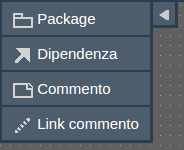
\includegraphics[scale=0.6]{./Immagini/AppToolbar.png}
					\caption{Interfaccia grafica - Esempio di toolbar}\label{fig:AppToolbar}
				\end{figure}
				\item \underline{Pannello delle proprietà} che compare alla selezione di un elemento nell'area di lavoro
				ed offre tutte le sue informazioni con la possibilità di modificarle (vedi Figura \ref{fig:AppEditPanel});
				\begin{figure} [h!]
					\centering
					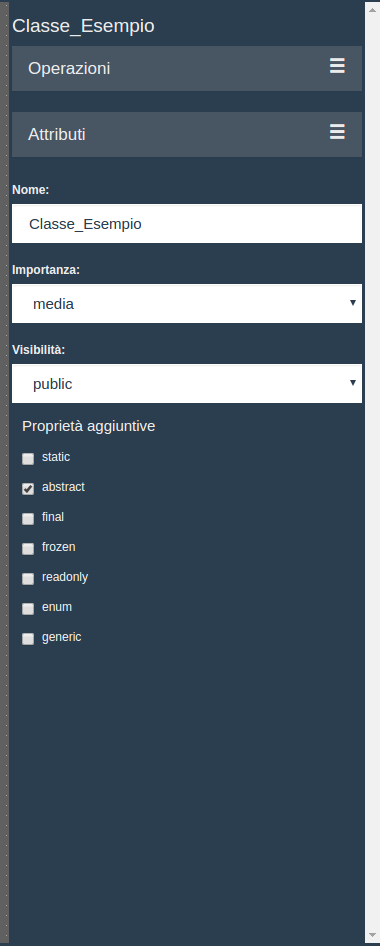
\includegraphics[scale=0.3]{./Immagini/AppEditPanel.png}
					\caption{Interfaccia grafica - Esempio di pannello delle proprietà}\label{fig:AppEditPanel}
				\end{figure}
				\item \underline{Percorso attuale} che visualizza la posizione corrente (il tipo di diagramma) tra i
				diagrammi del progetto (maggiori informazioni alla sezione \ref{sez:Path}).
			\end{enumerate}
			\subsubsection{Menù dell'applicazione}
				Il menù è sempre disponibile in qualunque posizione vi troviate all'interno
				dell'applicazione e al suo interno è possibile selezionare le seguenti voci:
				\begin{itemize}
					\item \textit{\textbf{File}}
					\begin{itemize}
						\item \textit{\textbf{Nuovo Progetto}}: elimina il contenuto dell'eventuale progetto
						correntemente aperto ripulendo l'area di lavoro: prima di procedere viene chiesto se si vuole
						salvare il progetto correntemente aperto attraverso una finestra di dialogo;
						\item \textit{\textbf{Apri}}: apre una finestra di dialogo per poter caricare un
						file di progetto salvato localmente nel proprio pc avente estensione ``.swed'';
						\item \textit{\textbf{Salva}}: salva il progetto correntemente aperto ed esegue il
						download in locale del relativo file con estensione ``.swed'';
						\item \textit{\textbf{Salva con nome}}: salva il progetto correntemente aperto, apre
						una finestra di dialogo per scegliere il nome da dare al file di progetto e ne esegue
						il download in locale.
					\end{itemize}
					\begin{figure} [h!]
						\centering
						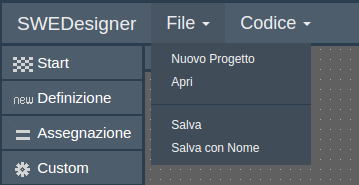
\includegraphics[scale=0.5]{./Immagini/AppFile.png}
						\caption{Menù dell'applicazione - Sezione ``File''}\label{fig:AppFile}
					\end{figure}
					\item \textit{\textbf{Codice}}
					\begin{itemize}
						\item \textit{\textbf{Genera Codice Java}}: invia una richiesta al server per generare
						il codice in linguaggio Java del progetto corrente e successivamente avvia il
						download del file compresso ``.zip'' contenente il/i file compilato/i; All'interno del file
						compresso è presente anche un file di testo ``report.txt'' contenente gli eventuali errori
						verificatisi durante la compilazione del codice generato;
						\item \textit{\textbf{Genera Codice Javascript}}: invia una richiesta al server per
						generare il codice in linguaggio Javascript del progetto corrente e successivamente
						avvia il download del file compresso ``.zip'' contenente il/i file di script.
					\end{itemize}
					\begin{figure} [h!]
						\centering
						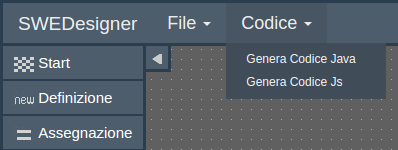
\includegraphics[scale=0.5]{./Immagini/AppCode.png}
						\caption{Menù dell'applicazione - Sezione ``Codice''}\label{fig:AppCode}
					\end{figure}
				\end{itemize}
			\subsubsection{Percorso attuale}\label{sez:Path}
				Il percorso attuale, sempre visibile in basso a sinistra dell'applicazione, visualizza la
				posizione corrente (il tipo di diagramma) tra i diagrammi del progetto.\\
				Da qui è possibile spostarsi verso un diagramma
				antecedente a quello attuale cliccandone il corrispondente link.
				\begin{figure} [h!]
					\centering
					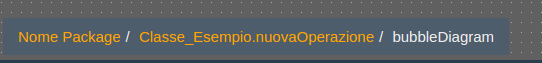
\includegraphics[scale=0.5]{./Immagini/AppPath.png}
					\caption{Interfaccia grafica - Esempio di percorso attuale}\label{fig:AppPath}
				\end{figure}
		\newpage
		\subsection{Editor del diagramma dei package}
			L'editor del diagramma dei package comparirà ad ogni apertura di un progetto o alla creazione di uno nuovo.
			È il punto di partenza per iniziare a progettare il vostro programma ed in esso è possibile gestirne
			l'architettura al più alto livello disponibile.
			\begin{figure} [h!]
				\centering
				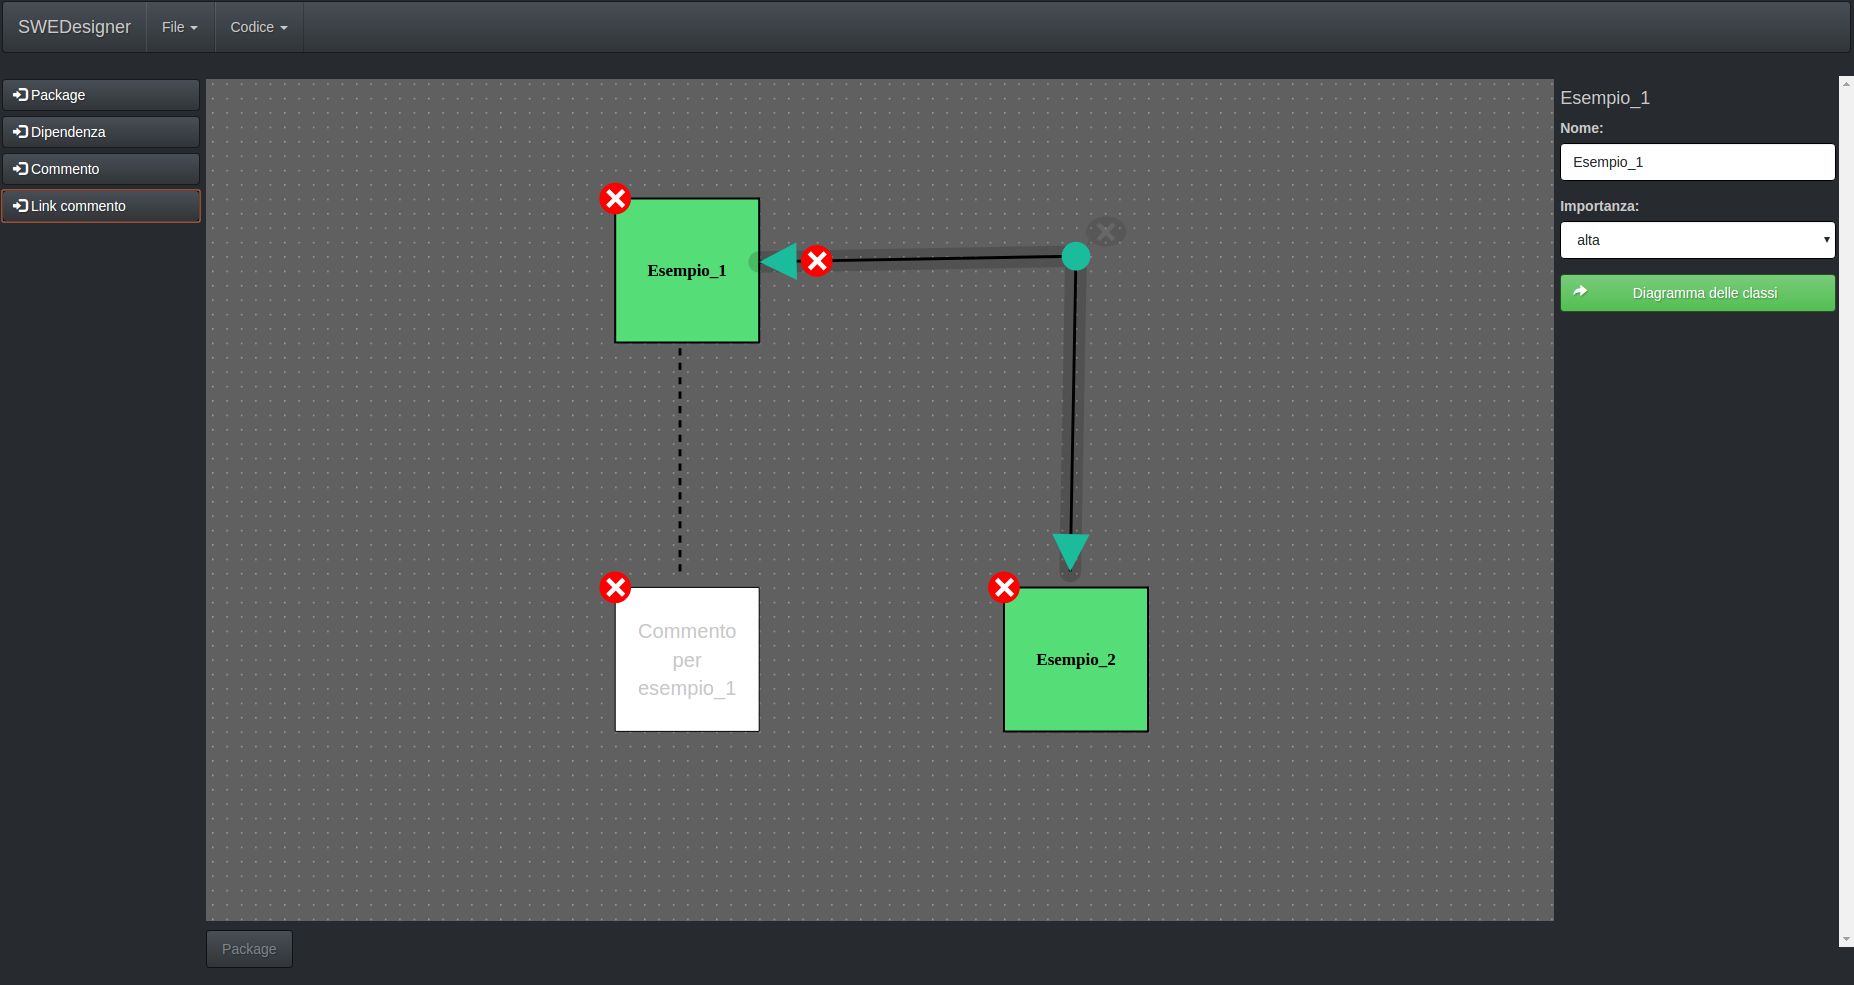
\includegraphics[scale=0.24]{./Immagini/PackageDiagram.png}
				\caption{Editor del diagramma dei package - esempio di sviluppo di diag. dei package}\label{fig:PackageDiagram}
			\end{figure}
			\subsubsection{Menù degli strumenti}
				Dal menù degli strumenti (vedi Figura \ref{fig:ToolbarPkgDiag}) potrete aggiungere i seguenti elementi
				al vostro diagramma:
				\begin{itemize}
					\item \textit{\textbf{Package}}: generalmente, il punto d'inizio nella creazione di un programma.\\
					Cliccare il pulsante e poi cliccare il luogo desiderato
					dell'area di lavoro per crearvi un package;
					\item \textit{\textbf{Dipendenza}}: quando alcuni componenti di un package dipendono dai componenti
					appartenenti ad un altro package del diagramma, dovrete segnalare una dipendenza.\\
					Cliccare il pulsante, cliccare il package sorgente
					(dipendente) e successivamente quello destinatario per creare una relazione di dipendenza;
					\item \textit{\textbf{Commento}}: se volete, potete aggiungere un commento UML per facilitare la
					comprensione del vostro diagramma.\\
					Cliccare il pulsante e poi cliccare il luogo desiderato
					dell'area di lavoro per crearvi un commento;
					\item \textit{\textbf{Link commento}}: quando creerete il vostro commento, potrete collegarlo
					all'elemento del diagramma a cui è rivolto utilizzando questo apposito collegamento.\\
					Cliccare il pulsante, cliccare il package ed il
					commento desiderati per collegarli.
				\end{itemize}
				\begin{figure} [h!]
					\centering
					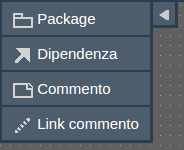
\includegraphics[scale=0.5]{./Immagini/ToolbarPkgDiag.png}
					\caption{Editor del diagramma dei package - toolbar}\label{fig:ToolbarPkgDiag}
				\end{figure}
				Per spostare un elemento (Package o Commento) all'interno dell'area di lavoro, cliccarlo con
				il mouse e trascinarlo verso la posizione desiderata.\\
				Per cambiare un membro di una relazione, trascinarne un apice sull'elemento
				desiderato.\\
				Per spezzare una relazione in un punto specifico della linea, eseguire un doppio click sulla
				posizione desiderata.\\
				Per eliminare un elemento dal diagramma, cliccare sulla rispettiva icona nell'area di lavoro
				avente una croce rossa (verrà visualizzata quando porterete il cursore sopra l'elemento in questione):
				comparirà un messaggio di richiesta di conferma e basterà cliccare il pulsante ``Ok'' per proseguire,
				``Annulla'' altrimenti.
			\subsubsection{Pannello delle proprietà}
				Come già descritto precedentemente, il pannello delle proprietà di un elemento del diagramma comparirà
				alla selezione dell'elemento stesso sull'area di lavoro.\\
				Al click dell'elemento desiderato, comparirà il corrispondente pannello delle sue proprietà sul lato
				destro dell'interfaccia. Inoltre, l'elemento correntemente selezionato, verrà evidenziato per permetterne
				un più facile riconoscimento all'interno del diagramma.\\
				Per modificare una qualunque proprietà testuale, editare il campo di testo e successivamente premere il
				tasto "Invio" della tastiera oppure cliccare altrove all'interno del pannello delle proprietà.\\
				Per modificare una proprietà non testuale, cambiare semplicemente il valore selezionando quello
				desiderato.\\
				Dopo la creazione di un package la prima cosa che si consiglia di fare, è cambiarne il nome che viene
				impostato di default. Per ciascun package, presente nel diagramma, è inoltre possibile impostarne
				l'importanza che cambia il colore dell'elemento facilitando la visualizzazione delle componenti
				che sono più importanti all'interno della vostra area di lavoro.
				I livelli di importanza selezionabili sono:
				\begin{itemize}
					\item \textbf{alta}: il package in questione si colora di rosso;
					\item \textbf{media}: il package in questione si colora in ocra (è l'impostazione di default);
					\item \textbf{bassa}: il package in questione si colora di bianco.
				\end{itemize}
				Nel pannello proprietà di ogni package, è presente il pulsante
				\textit{\textbf{Diagramma delle classi}}: premendolo vi sposterete al diagramma delle classi
				del package selezionato.
				Quando non avrete più bisogno del pannello, cliccate in una zona vuota dell'area di lavoro per farlo
				scomparire.
				\textbf{Nota informativa}: in Java, per importare dei package di linguaggio (ad es. java.util.ArrayList)
				create un package e rinominatelo adeguatamente (nel caso dell'esempio "java.util.ArrayList");
				dopodichè collegate i package che ne sono dipendenti con l'apposita relazione.
		\newpage
		\subsection{Editor del diagramma delle classi}
			Quando avrete creato un package e vorrete definirne il contenuto (classi e interfacce), potrete cliccare
			sul suo pulsante \textit{\textbf{Diagramma delle classi}}, descritto nella sezione precedente, che
			cambierà l'area di lavoro facendo visualizzare il diagramma delle classi corrispondente. La prima volta che
			vi sposterete al diagramma delle classi di un package appena creato, l'area di lavoro sarà chiaramente vuota.
			Se invece vi sposterete in un diagramma delle classi precedentemente editato, troverete il contenuto
			creato nella stessa posizione in cui l'avevate lasciato.
			\begin{figure} [h!]
				\centering
				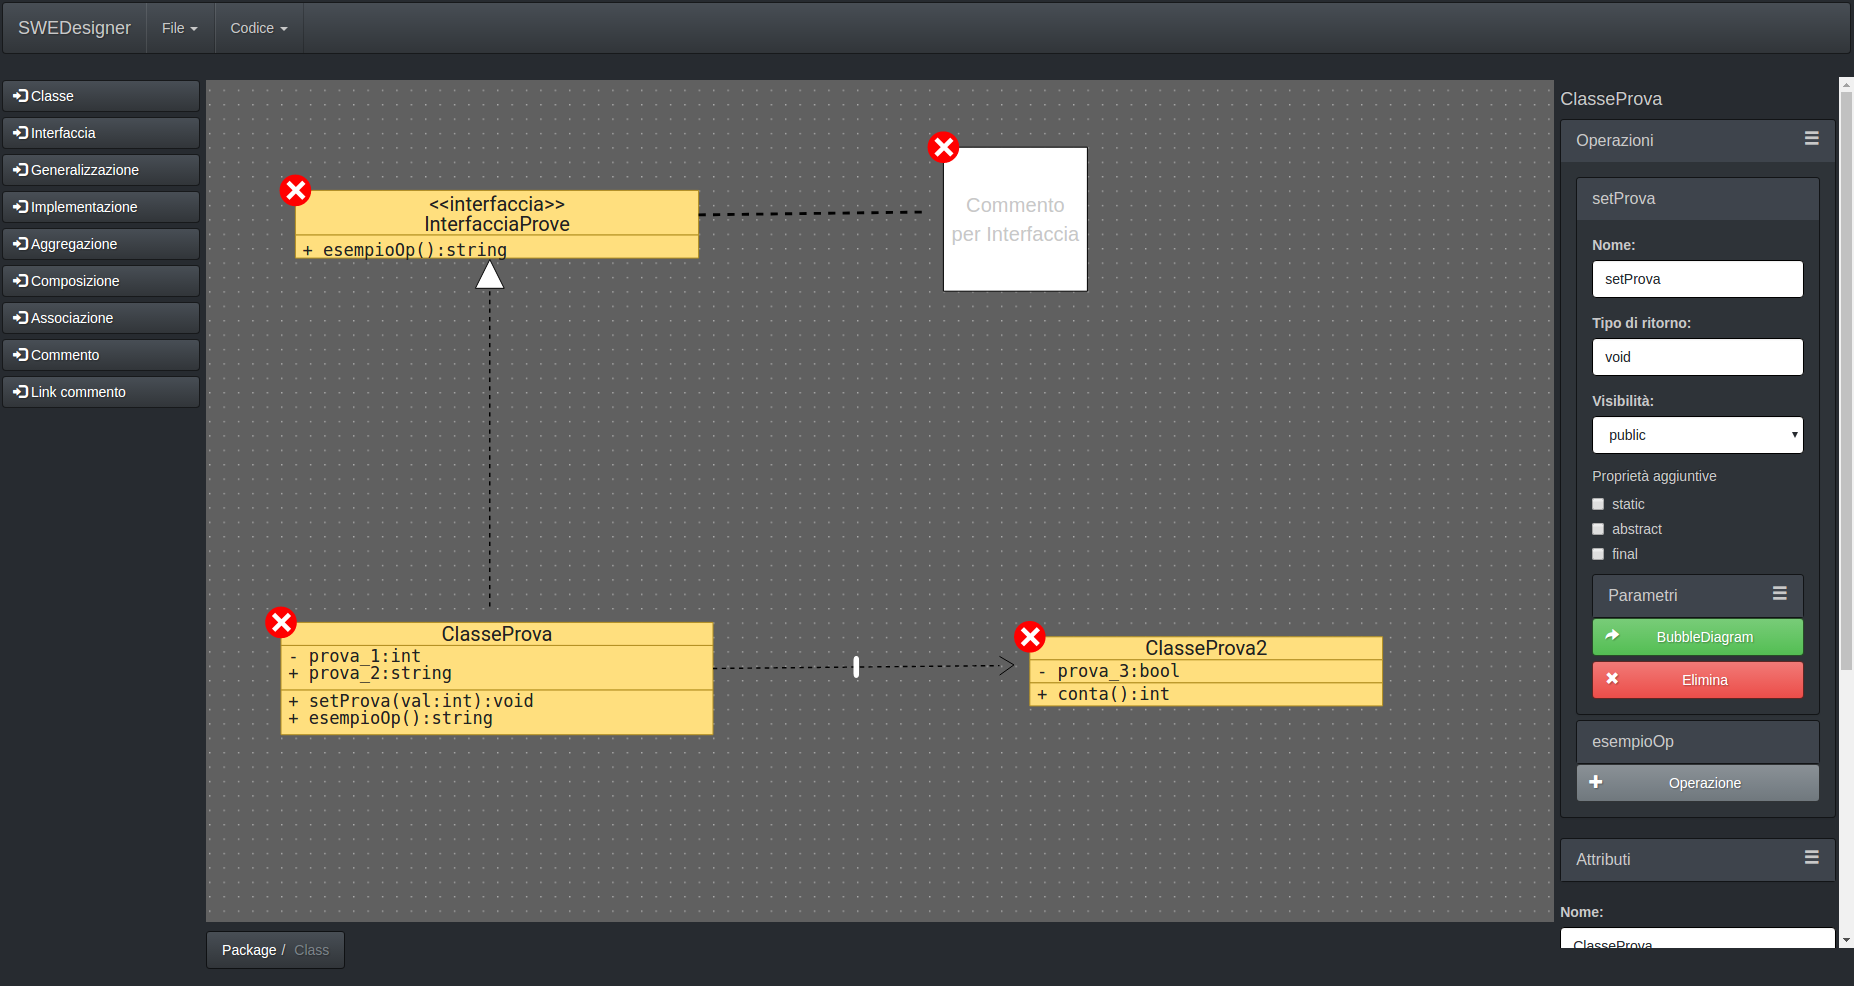
\includegraphics[scale=0.24]{./Immagini/ClassDiagram.png}
				\caption{Editor del diagramma delle classi - esempio di sviluppo di diag. delle classi}\label{fig:ClassDiagram}
			\end{figure}
			\subsubsection{Menù degli strumenti}
				Dal menù degli strumenti (vedi Figura \ref{fig:ToolbarClDiag}) potrete aggiungere i seguenti elementi
				al vostro diagramma:
				\begin{itemize}
					\item \textit{\textbf{Classe}}: cliccare il pulsante e poi cliccare il luogo desiderato
					dell'area di lavoro per crearvi una classe;
					\item \textit{\textbf{Interfaccia}}: cliccare il pulsante e poi cliccare il luogo desiderato
					dell'area di lavoro per crearvi un'interfaccia;
					\item \textit{\textbf{Generalizzazione}}: cliccare il pulsante, cliccare l'elemento sorgente
					e successivamente quello destinatario per creare una relazione di generalizzazione;
					\item \textit{\textbf{Implementazione}}: cliccare il pulsante, cliccare l'elemento sorgente
					e successivamente quello destinatario per creare una relazione di implementazione;
					\item \textit{\textbf{Aggregazione}}: cliccare il pulsante, cliccare l'elemento sorgente
					e successivamente quello destinatario per creare una relazione di aggregazione;
					\item \textit{\textbf{Composizione}}: cliccare il pulsante, cliccare l'elemento sorgente
					e successivamente quello destinatario per creare una relazione di composizione;
					\item \textit{\textbf{Associazione}}: cliccare il pulsante, cliccare l'elemento sorgente
					e successivamente quello destinatario per creare una relazione di associazione;
					\item \textit{\textbf{Commento}}: se volete, potete aggiungere un commento UML per facilitare la
					comprensione del vostro diagramma.\\
					Cliccare il pulsante e poi cliccare il luogo desiderato
					dell'area di lavoro per crearvi un commento;
					\item \textit{\textbf{Link commento}}: quando creerete il vostro commento, potrete collegarlo
					all'elemento del diagramma a cui è rivolto utilizzando questo apposito collegamento.\\
					Cliccare il pulsante, cliccare l'elemento ed il
					commento desiderati per collegarli.
				\end{itemize}
				\begin{figure} [h!]
					\centering
					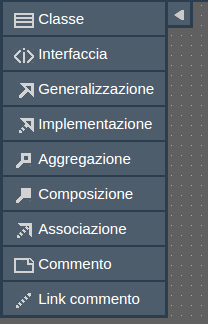
\includegraphics[scale=0.4]{./Immagini/ToolbarClDiag.png}
					\caption{Editor del diagramma delle classi - toolbar}\label{fig:ToolbarClDiag}
				\end{figure}
				Per spostare un elemento (Classe, Interfaccia o Commento) all'interno dell'area di lavoro,
				cliccarlo con il mouse e trascinarlo verso la posizione desiderata.\\
				Per cambiare un membro di una relazione, trascinarne un apice sull'elemento
				desiderato.\\
				Per "spezzare" una relazione in un punto specifico della linea, eseguire un doppio click sulla
				posizione desiderata.\\
				Per eliminare un elemento dal diagramma, cliccare sulla rispettiva icona nell'area di lavoro
				avente una croce rossa (verrà visualizzata quando porterete il cursore sopra l'elemento in questione):
				comparirà un messaggio di richiesta di conferma e basterà cliccare il pulsante ``Ok'' per proseguire,
				``Annulla'' altrimenti.
			\subsubsection{Pannello delle proprietà}
				Anche quando vi troverete in questo diagramma, al click dell'elemento desiderato, comparirà il
				corrispondente pannello delle sue proprietà sul lato destro dell'interfaccia.
				Inoltre, l'elemento correntemente selezionato, verrà evidenziato per permetterne
				un più facile riconoscimento all'interno del diagramma.\\
				Per modificare una proprietà testuale, editare il campo di testo e successivamente premere il
				tasto "Invio" della tastiera oppure cliccare altrove all'interno del pannello delle proprietà.\\
				Per modificare una proprietà non testuale, cambiare semplicemente il valore selezionando quello
				desiderato.\\
				Una volta creata e selezionata una classe, potrete aggiungere/modificare/eliminare attributi direttamente
				dal pannello: selezionare il pulsante \textit{\textbf{Attributi}} ed il pulsante
				\textit{\textbf{+ Attributo}}. Cliccando poi sul nome di un attributo della lista, compariranno i
				corrispondenti dettagli (nome, tipo, visibilità, ecc.) che potranno essere editati (per eliminare
				l'operazione selezionata basta cliccare sul corrispondente pulsante
				\textit{\textbf{Elimina}}).
				Dualmente, una volta creata e selezionata una classe (o interfaccia), potrete
				aggiungere/modificare/eliminare operazioni: selezionare il pulsante \textit{\textbf{Operazioni}} ed il
				pulsante \textit{\textbf{+ Operazione}}. Cliccando poi sul nome di un'operazione della lista,
				compariranno i corrispondenti dettagli (nome, tipo di ritorno, visibilità, ecc.) che potranno essere
				editati (per eliminare l'operazione selezionata basta cliccare sul corrispondente pulsante
				\textit{\textbf{Elimina}}); dalla medesima sezione di dettaglio è possibile
				aggiungere/modificare/eliminare i parametri con una procedura simile a quella usata per gestire
				operazioni e attributi.
				Nel pannello proprietà delle classi, per ogni sotto-pannello di operazione definita,
				è possibile spostarsi al rispettivo diagramma delle bubble premendo il relativo pulsante
				\textit{\textbf{BubbleDiagram}}.
				Quando non avrete più bisogno del pannello, cliccate in una zona vuota dell'area di lavoro per farlo
				scomparire.
		\newpage
		\subsection{Editor del diagramma delle bubble}\label{sez:BubbleDiagram}
			Quando avete creato una classe e ne avete definito un'operazione potrete andare a realizzarla spostandovi al
			corrispondente diagramma delle bubble premendo il relativo pulsante descritto nella sezione precedente.
			Nel diagramma delle bubble è possibile quindi strutturare ed ordinare i passi da compiere di un'operazione.
			Questo tipo di diagramma è stato ideato dal team di sviluppo di \progetto\
			e si discosta dai diagrammi UML di attività e sequenza. Tende piuttosto ad assomigliare ad un
			flow-chart.\\
			Una bubble è un elemento del diagramma e rispecchia una determinata istruzione (o set di
			istruzioni) traducibili in codice sorgente (condizione, ciclo, ...).\\
			È possibile realizzare set di istruzioni definite da bubble innestandole tra loro\footnote{Maggiori informazioni alla definizione dello strumento \textit{\textbf{Innesta}}, nella sezione \ref{sez:BubbleDiagram-strumenti}}.
			Ogni diagramma delle bubble è caratterizzato da una bubble \textit{\textbf{Start}} che segna
			il punto d'inizio dell'operazione.
			\begin{figure} [h!]
				\centering
				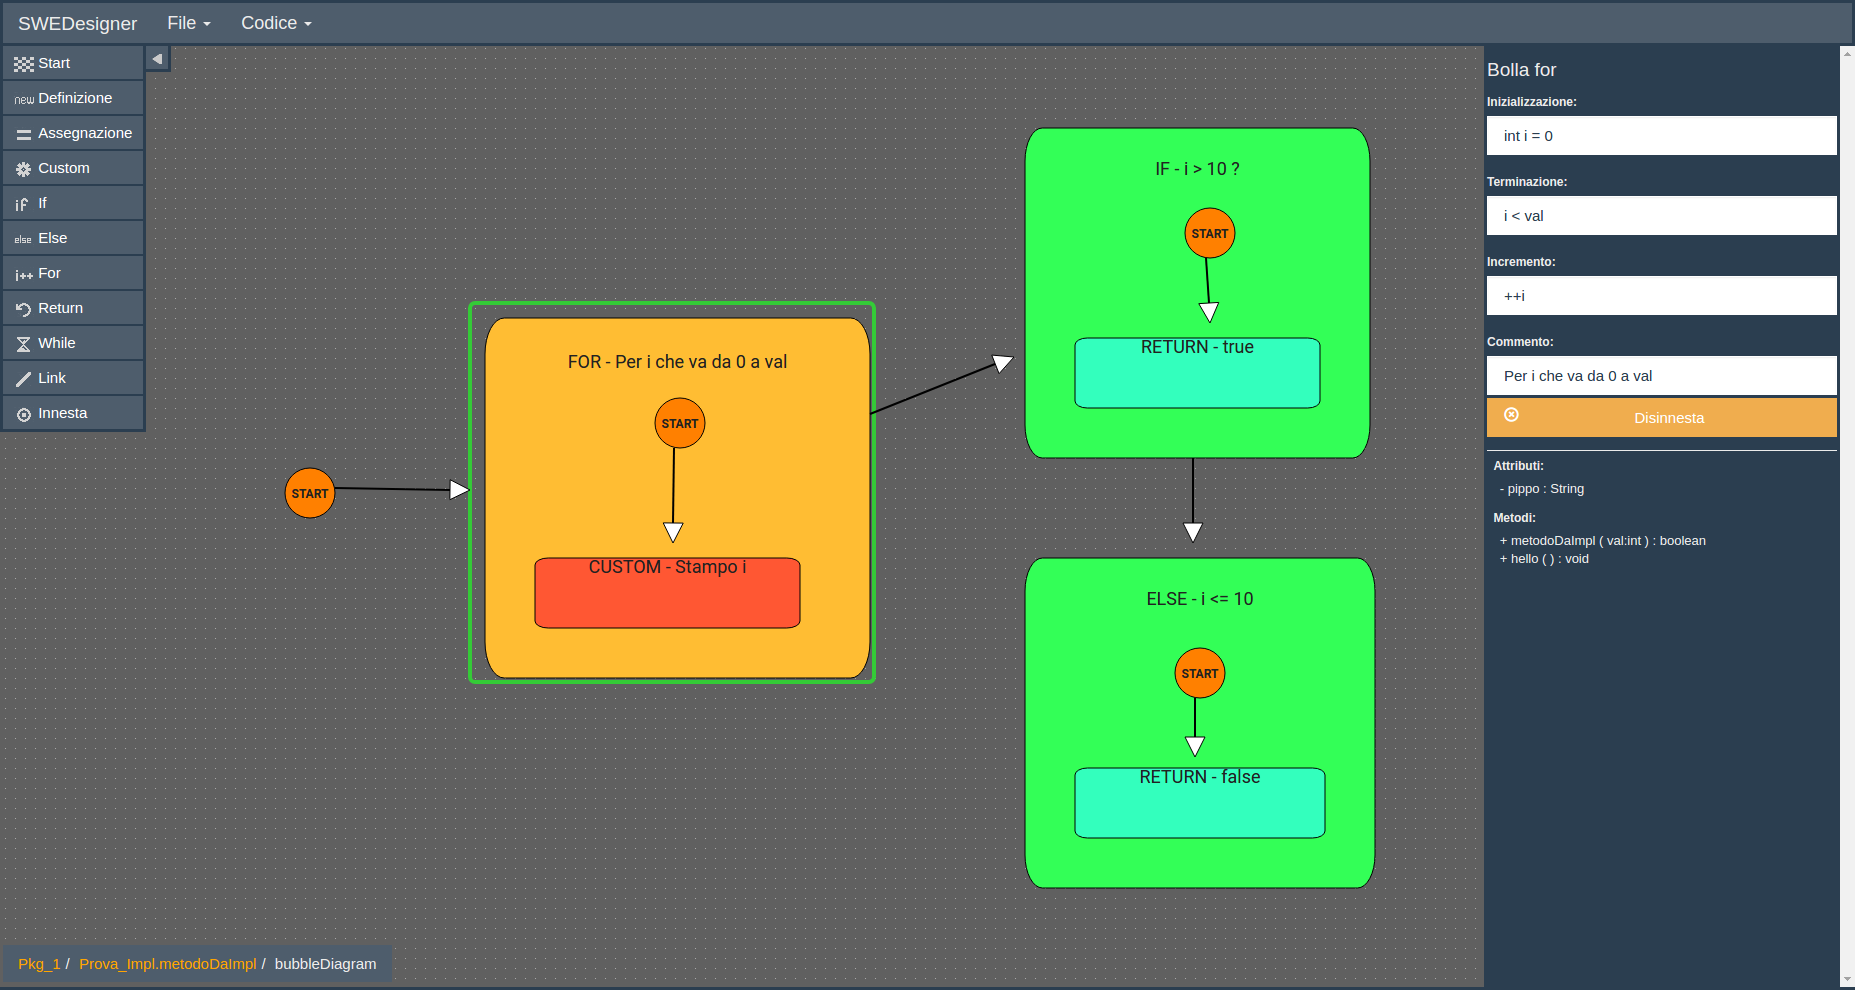
\includegraphics[scale=0.24]{./Immagini/BubbleDiagram.png}
				\caption{Editor del diagramma delle bubble - esempio di sviluppo di operazione}\label{fig:BubbleDiagram}
			\end{figure}
			\subsubsection{Menù degli strumenti}\label{sez:BubbleDiagram-strumenti}
				Le diverse bubble inseribili (vedi Figura \ref{fig:ToolbarBubbleDiag}) nel diagramma sono:
				\begin{itemize}
					\item \textit{\textbf{Start}}: specifica il punto di inizio dell'algoritmo che si sta
					sviluppando. Deve essere inserita anche per indicare il punto iniziale di un blocco di bubble
					innestate tra loro (vedi bolle For, If, Else presenti nell'esempio in Figura
					\ref{fig:BubbleDiagram}).\\
					Per crearla, cliccare il pulsante e poi cliccare il luogo desiderato
					dell'area di lavoro;
					\item \textit{\textbf{Definizione}}: corrisponde ad uno statement di definizione di variabile,
					dove è possibile impostarne tipo, nome e valore iniziale (opzionale).\\
					Per crearla, cliccare il pulsante e poi cliccare il luogo desiderato
					dell'area di lavoro;
					\item \textit{\textbf{Assegnazione}}: corrisponde ad uno statement di tipo "x = y;", dove è
					possibile impostare cosa vale "x" e cosa "y".\\
					Per crearla, cliccare il pulsante e poi cliccare il luogo desiderato
					dell'area di lavoro;
					\item \textit{\textbf{Custom}}: al suo interno, potrete definire un insieme di istruzioni
					(dallo specifico pannello delle proprietà in due campi di testo ognuno per il corrispondente
					linguaggio di possibile generazione) che saranno copiate nel codice sorgente generato.\\
					Per crearla, cliccare il pulsante e poi cliccare il luogo desiderato
					dell'area di lavoro;
					\item \textit{\textbf{If}}: corrisponde all'istruzione condizionale ``if''; specifica un blocco
					di bubble (da innestare) eseguibili al verificarsi di una condizione.\\
					Per crearla, cliccare il pulsante e poi cliccare il luogo desiderato
					dell'area di lavoro;
					\item \textit{\textbf{Else}}: corrisponde all'istruzione condizionale ``else''; specifica un
					blocco di bubble (da innestare) eseguibili alternativamente al non	verificarsi di una
					condizione.\\
					Per crearla, cliccare il pulsante e poi cliccare il luogo desiderato
					dell'area di lavoro;
					\item \textit{\textbf{For}}: corrisponde all'istruzione iterativa ``for''; specifica un
					blocco di bubble (da innestare) la cui esecuzione verrà ripetuta fino al verificarsi della
					condizione impostata.\\
					Per crearla, cliccare il pulsante e poi cliccare il luogo desiderato
					dell'area di lavoro;
					\item \textit{\textbf{Return}}: corrisponde all'istruzione ``return''; definisce la variabile
					o un valore da ritornare.\\
					Per crearla, cliccare il pulsante e poi cliccare il luogo desiderato
					dell'area di lavoro;
					\item \textit{\textbf{While}}: specifica un blocco di bubble (da innestare) la cui esecuzione
					verrà ripetuta fino al verificarsi della condizione impostata.\\
					Per crearla, cliccare il pulsante e poi cliccare il luogo desiderato
					dell'area di lavoro;
					\item \textit{\textbf{Link}}: specifica l'ordine di esecuzione tra due bubble.\\
					Per crearla, cliccare il pulsante, cliccare l'elemento antecedente
					e successivamente quello successivo per creare una relazione di esecuzione sequenziale;
					\item \textit{\textbf{Innesta}}: utilizzabile per innestare una bubble dentro l'altra.
					In un concetto di semplice esecuzione dell'operazione in sviluppo, la
					logica della struttura del codice di bubble innestate è la seguente:
					\begin{enumerate}
						\item Prima viene eseguito il codice definito nella bubble innestante (ad esempio,
						condizione ``if``, controllo di ciclo ``while'', ...);
						\item All'interno del blocco definito nella bubble innestante viene eseguito il codice
						definito sequenzialmente a partire dalla bubble \textit{\textbf{Start}}.
					\end{enumerate}
					È possibile effettuare molteplici annidamenti.\\
					Per innestare, cliccare il pulsante, cliccare la specifica bubble
					e successivamente la bubble contenitrice;
				\end{itemize}
				\begin{figure} [h!]
					\centering
					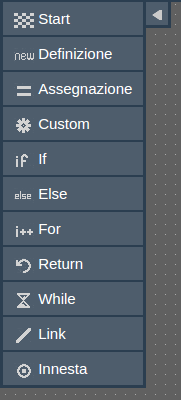
\includegraphics[scale=0.36]{./Immagini/ToolbarBubbleDiag.png}
					\caption{Editor del diagramma delle bubble - toolbar}\label{fig:ToolbarBubbleDiag}
				\end{figure}
				Per spostare una bubble all'interno dell'area di lavoro,
				cliccarla con il mouse e trascinarla verso la posizione desiderata.\\
				Per cambiare un membro di una relazione, trascinarne un apice sull'elemento
				desiderato.\\
				Per "spezzare" un link in un punto specifico della linea, eseguire un doppio click sulla
				posizione desiderata.\\
				Per eliminare un elemento dal diagramma, cliccare sulla rispettiva icona nell'area di lavoro
				avente una croce rossa (verrà visualizzata quando porterete il cursore sopra l'elemento in
				questione): comparirà un messaggio di richiesta di conferma e basterà cliccare il pulsante ``Ok'' per
				proseguire, ``Annulla'' altrimenti.
				\textbf{ATTENZIONE}: Eliminando una bubble contenente al suo interno altre bubble innestate,
				eliminerete anch'esse.
			\subsubsection{Pannello delle proprietà}
				Cliccando su un elemento del diagramma delle bubble esso verrà evidenziato come descritto
				per i diagrammi di package e classi; inoltre, verrà visualizzato il corrispondente pannello
				di dettaglio contenente tutte le proprietà modificabili dell'elemento stesso.\\
				Per modificare una proprietà testuale, editare il campo di testo e successivamente premere il
				tasto "Invio" della tastiera oppure cliccare altrove all'interno del pannello delle proprietà.
				Per le bubble \textit{\textbf{Custom}}, una volta terminato di inserire il codice nell'apposito spazio,
				potrete seguire ciò scritto sopra oppure premere il pulsante \textit{\textbf{Salva codice}}.\\
				Per modificare una proprietà non testuale, cambiare semplicemente il valore selezionando quello
				desiderato.\\
				Nel caso in cui doveste disinnestare una bubble precedentemente innestata sarà sufficiente aprire il
				corrispondente pannello delle proprietà e cliccare sul pulsante \textit{\textbf{Disinnesta}}.\\
				Per riconoscere più facilmente il significato di una bubble all'interno del grafo, è possibile
				assegnarvi un commento dal relativo pannello delle proprietà (campo ``Commento'').\\
				In ogni pannello delle proprietà è rappresentata una lista di descrizione degli attributi e dei
				metodi della classe su cui si sta lavorando (vedi Figura \ref{fig:ClassDesc}) per facilitare la
				visione del contesto in cui si trova l'operazione in corso d'opera.
				\begin{figure} [h!]
					\centering
					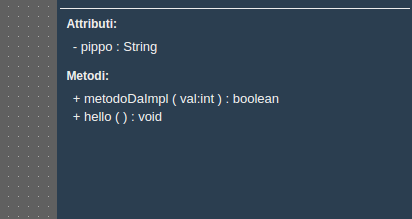
\includegraphics[scale=0.4]{./Immagini/ClassDesc.png}
					\caption{Lista di descrizione delle componenti di una classe}\label{fig:ClassDesc}
				\end{figure}
\end{document}
